\documentclass[preprint,12pt]{elsarticle}
% \documentclass[draft,12pt]{elsarticle}

\usepackage{hyperref}
\usepackage{graphicx}
\usepackage{subcaption}
\usepackage{amssymb}
\usepackage{amsmath}
\usepackage{multirow}
\usepackage{relsize}
\usepackage[utf8]{inputenc}
\usepackage[capitalise]{cleveref}
\usepackage{algorithm}
\usepackage[noend]{algpseudocode}
\usepackage[section]{placeins}
\usepackage{booktabs}
\usepackage{url}

% For the TODOs
\usepackage{xcolor}
\usepackage{xargs}
\usepackage[colorinlistoftodos,textsize=footnotesize]{todonotes}
\newcommand{\todoin}{\todo[inline]}
% from here: https://tex.stackexchange.com/questions/9796/how-to-add-todo-notes
\newcommandx{\unsure}[2][1=]{\todo[linecolor=red,backgroundcolor=red!25,bordercolor=red,#1]{#2}}
\newcommandx{\change}[2][1=]{\todo[linecolor=blue,backgroundcolor=blue!25,bordercolor=blue,#1]{#2}}
\newcommandx{\info}[2][1=]{\todo[linecolor=OliveGreen,backgroundcolor=OliveGreen!25,bordercolor=OliveGreen,#1]{#2}}

%Boldtype for greek symbols
\newcommand{\teng}[1]{\ensuremath{\boldsymbol{#1}}}
\newcommand{\ten}[1]{\ensuremath{\mathbf{#1}}}

\usepackage{lineno}
% \linenumbers

\journal{}

\begin{document}

\begin{frontmatter}

  \title{{DEM}-{SPH} study of particles dispersion in fluid}
  \author[XXX]{Dinesh Adepu\corref{cor1}}
  \ead{d.dinesh@surrey.ac.uk}
  \author[University of Surrey]{Chuan Yu Wu}
  \ead{XXX}
\address[xxx]{xxx}

\cortext[cor1]{Corresponding author}


\begin{abstract}

\end{abstract}

\begin{keyword}
%% keywords here, in the form: keyword \sep keyword
{particle dispersion}, {particle mixing}, {SPH-DEM}, {stirrer}

%% MSC codes here, in the form: \MSC code \sep code
%% or \MSC[2008] code \sep code (2000 is the default)

\end{keyword}

\end{frontmatter}

% \linenumbers


\FloatBarrier%
\section{Introduction}


\subsection*{About swelling in real life}

Process engineering has food processing, detergents and many more. In the
formulations to improve quality and shelf life hydrocolids are
used. Hydrocollids when mixed with water undergoes water induced
diffusion. Hydrocolloids are used in food processing as thckening agents and
gelling agents. Due to hydocollids being hydrophillic they absorb water and
swell. The swelling of hydrocolloids, adhesion, affets the viscosity
surrounding, it results in the flow behaviour change. Used in many food
products. Basic hydrocolloids properties in floods are thickening, gelling,
emulsifying, stabilisation and controlling the crystal growth of ice and
sugar.


% Rubber particles swelling \cite{wang2019numerical}. Recently, the emerging
% hydrothermal treatment of waste plastics into clean fuel and chemical raw
% materials has been widely concerned. Process industry, has lot of particle
% swelling due to diffusion of fluid in the particles. Especially hydrocolloids
% are used as thickener agents.

\subsection*{Swelling modeling and study in experiments and numerical}

\begin{itemize}
\item Many researchers carried out experimental investigation on the water
  absorption of biological materials during isothermal soaking
  \cite{kashaninejad2007study,shittu2012physical}, and a few studies also
  aimed to examine the volume expansion associated with the water uptake
  during isothermal \cite{perez2012modeling} and non-isothermal treatments
  \cite{palanisamy2020kinetic}.

\item

\item \cite{braile2022analysis} studied the swelling of granular systems using
  DEM with a first order kinetic swelling model. SAP particles are studied in
  the paper.
\item First say, CFD-DEM and SPH-DEM are used to model several mixing
  problems. Discuss their drawbacks and advantages.
\item Now mention swelling has been introduced in CFD-DEM model.
\end{itemize}



\begin{itemize}
\item Crumb rubber modified bitumen (CRMB) swelling is studied using FEM
  \cite{wang2019numerical}.
\end{itemize}


\subsection*{Drawbacks of the existing numerical techniques in modeling
  swelling and other drawbacks. Why SPH and meshless techniques are better.}
Our SPH-DEM model is fully resolved, while CFD-DEM proposed in Hu 2023 is
unresolved coupling where, drag laws are used to compute the force on the
particles due to the interaction with the fluid.

\subsection*{What will we do in this current work and tools used}

\subsection*{Summary of the paper}





\FloatBarrier%
\section{Numerical modeling}


\subsection*{Fluid modeling}

% \subsection{Discretized fluid governing equations}
The SPH discretization of the continuity
equation~\cref{eq:sph-discretization-continuity} is given as,
\begin{equation}
  \label{eq:sph-discretization-continuity}
  \frac{{d}\rho_a}{dt} = \sum_{b} \; \frac{m_b}{\rho_{b}} \;
  \rho_{a} \; {\ten{u}}_{ab} \; \cdot \nabla_{a} W_{ab},
\end{equation}

%
Similarly, the discretized momentum equation is written as,
\begin{multline}
  \label{eq:sph-momentum-fluid}
  \frac{{d}\ten{u}_{a}}{dt} = - \sum_{b} m_b
  \bigg(\frac{p_a}{\rho_a^2} + \frac{p_b}{\rho_b^2}\bigg)
  \nabla_{a} W_{ab}
 \;+\;
  \sum_{b} m_b \frac{4 \eta \nabla W_{ab}\cdot
    \ten{r}_{ab}}{(\rho_a + \rho_b) (r_{ab}^2 + 0.01 h_{ab}^2)} \ten{u}_{ab}  \;+\;
  \ten{g}_{a},
\end{multline}
where $\ten{I}$ is the identity matrix, $\eta$ is the kinematic viscosity of the
fluid. The viscous term in \Cref{eq:me} is discretized according to the
formulation introduced in \cite{morris1997modeling}.

We add to the momentum equation an additional artificial viscosity term
$\Pi_{ab}$~\cite{monaghan-review:2005} to maintain the stability of the
numerical scheme, given as,
\begin{align}
  \label{eq:mom-av}
  \Pi_{ab} =
  \begin{cases}
\frac{-\alpha h_{ab} \bar{c}_{ab} \phi_{ab}}{\bar{\rho}_{ab}}
  & \ten{u}_{ab}\cdot \ten{r}_{ab} < 0, \\
  0 & \ten{u}_{ab}\cdot \ten{r}_{ab} \ge 0,
\end{cases}
\end{align}
where,
%
\begin{equation}
  \label{eq:av-phiij}
  \phi_{ab} = \frac{\ten{u}_{ab} \cdot \ten{r}_{ab}}{r^2_{ab} + 0.01 h^2_{ab}},
\end{equation}
%
where $\ten{r}_{ab} = \ten{r}_a - \ten{r}_b$,
$\ten{u}_{ab} = \ten{u}_a - \ten{u}_b$, $h_{ab} = (h_a + h_b)/2$,
$\bar{\rho}_{ab} = (\rho_a + \rho_b)/2$, $\bar{c}_{ab} = (c_a + c_b) / 2$, and
$\alpha$ is the artificial viscosity parameter.  The pressure $p_a$ is evaluated
using an equation of state:
\begin{equation}
\label{eqn:sph-eos}
  p_a = K \bigg(\frac{\rho_a}{\rho_{0}} - 1 \bigg).
\end{equation}
Where, $K=\rho_0 \, c_0^2$ is bulk modulus of the body, with
$c_0=10 \times V_{\text{max}}$ is speed of sound, while $\rho_0$ as the
initial density of the particles.

\subsection*{DEM}

\subsection*{Rigid-fluid coupling}

\subsection*{Swelling model}

\begin{equation}
\label{eqn:young_swelling_change}
\frac{\partial c}{\partial t} = \frac{D}{r^2}\frac{\partial}{\partial r}\bigg(r^2 \frac{\partial c}{\partial r}\bigg)
\end{equation}

With variable diffusion coefficient, \cite{dutta2020numerical},
\begin{equation}
\label{eqn:shear_swelling_change}
  D = D_0 exp^{\delta c / c_max}
\end{equation}
\todo{Define the variables}

The mass transfer rate during water diffusion can be calculated using the mass
balance equation \cite{kimber2013formulation},
\begin{equation}
\label{eqn:mass-balance-equation-swelling}
\frac{d m_w}{d t} = \dot{m}_{lp} + \dot{m}_{pp}
\end{equation}


Total mass of water at (\textit{i} + 1) incremental time step,
\begin{equation}
\label{eqn:mass-increase}
m_w^{i+1} = m_w^{i} + \Delta m_w^{i+1}
\end{equation}


\begin{equation}
\label{eqn:mass-influx-lp}
\dot{m}_{lp} = \frac{S_p D (c_{w, l} - c^i_{w, p})}{r^i_p}
\end{equation}


\begin{equation}
\label{eqn:mass-influx-pp}
\dot{m}_{pp} = \sum_{b \neq a} S_{ab} D_{pp} (c_{w, b} - c_{w, a})/r_{con}
\end{equation}

\begin{equation}
\label{eqn:volume-of-water-in-particle}
{V}_{w}^{i+1} = \frac{m_w^{i + 1}}{\rho_w}
\end{equation}
$\rho_w$ is the mass density ofthe water.

Then the instantaneous volume of the swollen particle ${V}_{w}^{i+1}$ is
determined as the sum of the initial volume of the dry particle $V_p^0$ and
the volume of water transferred into the particle $V_w^{i+1}$

\begin{equation}
\label{eqn:volume-of-water-in-particle}
{V}_{p}^{i+1} = {V}_{p}^{0} + {V}_{w}^{i+1}
\end{equation}

Therefore, the instantaneous radius of the particle at the $(i + 1)$the
timestep  ${r}_{p}^{i+1}$ is determined as
\begin{equation}
\label{eqn:volume-of-water-in-particle}
{r}_{p}^{i+1} = (3 {V}_{p}^{i+1} / 4 \pi)^{1 / 3}
\end{equation}



\subsubsection*{Macroscopic swelling model}
Change in mechanical properties \cite{sweijen2017grain}.


\begin{equation}
\label{eqn:shear_swelling_change}
  G_p^i = \frac{G_p^i}{\sqrt[3]{Q^i}}
\end{equation}

\begin{equation}
\label{eqn:young_swelling_change}
  E_p^i = \frac{E_p^i}{\sqrt[3]{Q^i}}
\end{equation}


\begin{equation}
\label{eqn:young_swelling_change}
  Q^i = \frac{m_p^i}{m_p^0}
\end{equation}

\subsubsection*{Material properties change due to swelling}
Change in mechanical properties \cite{sweijen2017grain}.


\begin{equation}
\label{eqn:shear_swelling_change}
  G_p^i = \frac{G_p^i}{\sqrt[3]{Q^i}}
\end{equation}

\begin{equation}
\label{eqn:young_swelling_change}
  E_p^i = \frac{E_p^i}{\sqrt[3]{Q^i}}
\end{equation}


\begin{equation}
\label{eqn:young_swelling_change}
  Q^i = \frac{m_p^i}{m_p^0}
\end{equation}




\begin{figure}[!htpb]
  \centering
  \begin{subfigure}{0.48\textwidth}
    \centering
    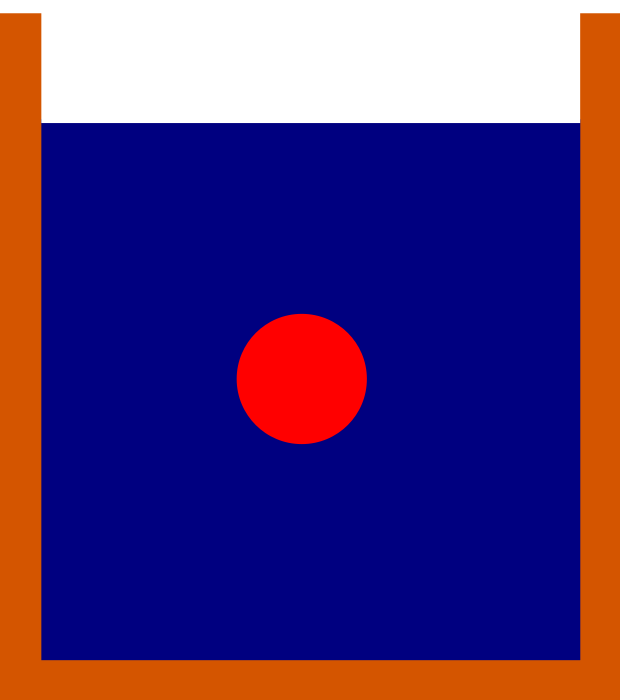
\includegraphics[width=0.45\textwidth]{images/hs_tank_with_spherical_particles_real_0_3}
    \subcaption{t = $3$ s}\label{fig:1-mixing-1-a}
  \end{subfigure}
  \begin{subfigure}{0.48\textwidth}
    \centering
    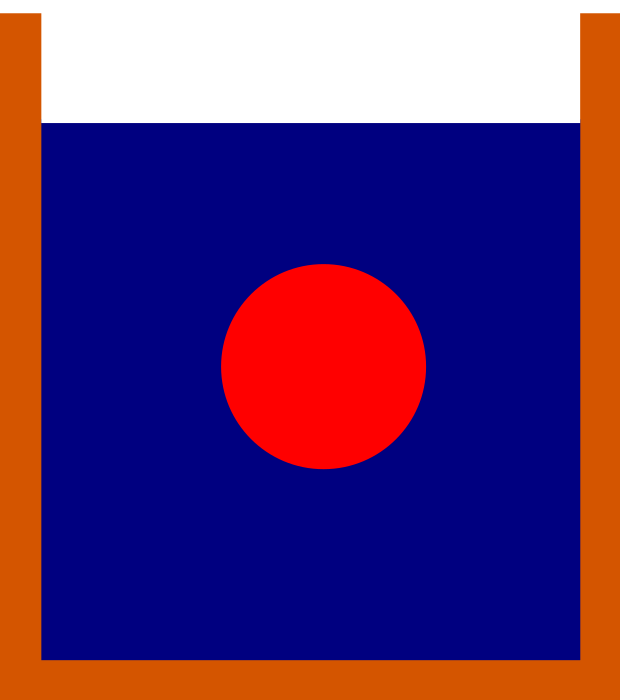
\includegraphics[width=0.45\textwidth]{images/hs_tank_with_spherical_particles_real_0_6}
    \subcaption{t = $6$ s}\label{fig:1-mixing-1-b}
  \end{subfigure}

  \begin{subfigure}{0.48\textwidth}
    \centering
    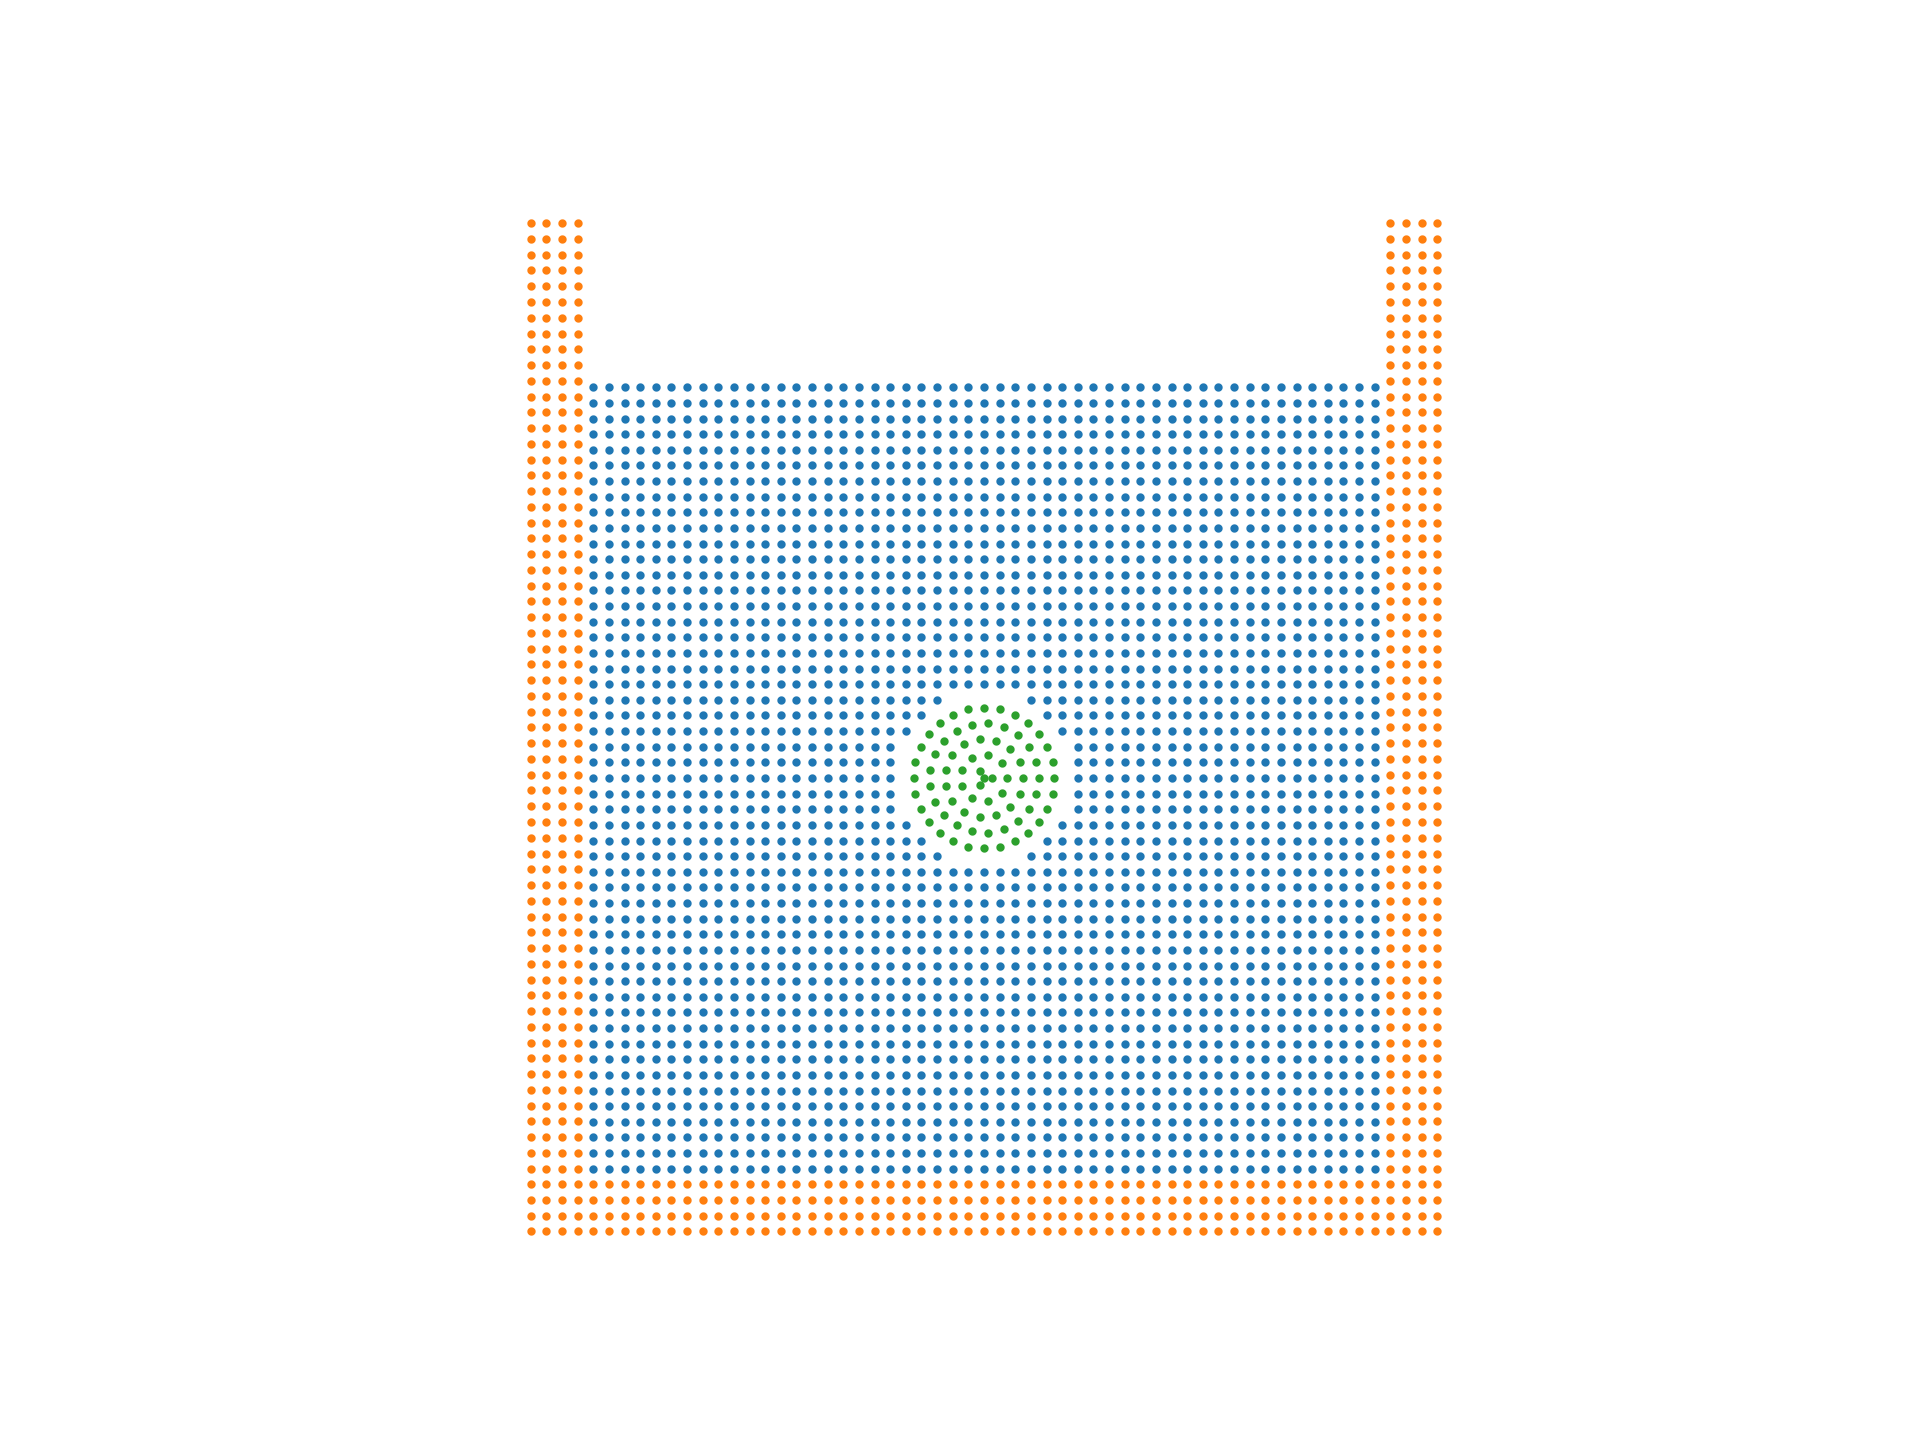
\includegraphics[width=1.0\textwidth]{images/hs_tank_with_spherical_particles_sph_0_3}
    \subcaption{t = $9.9$ s}\label{fig:1-mixing-1-c}
  \end{subfigure}
  \begin{subfigure}{0.48\textwidth}
    \centering
    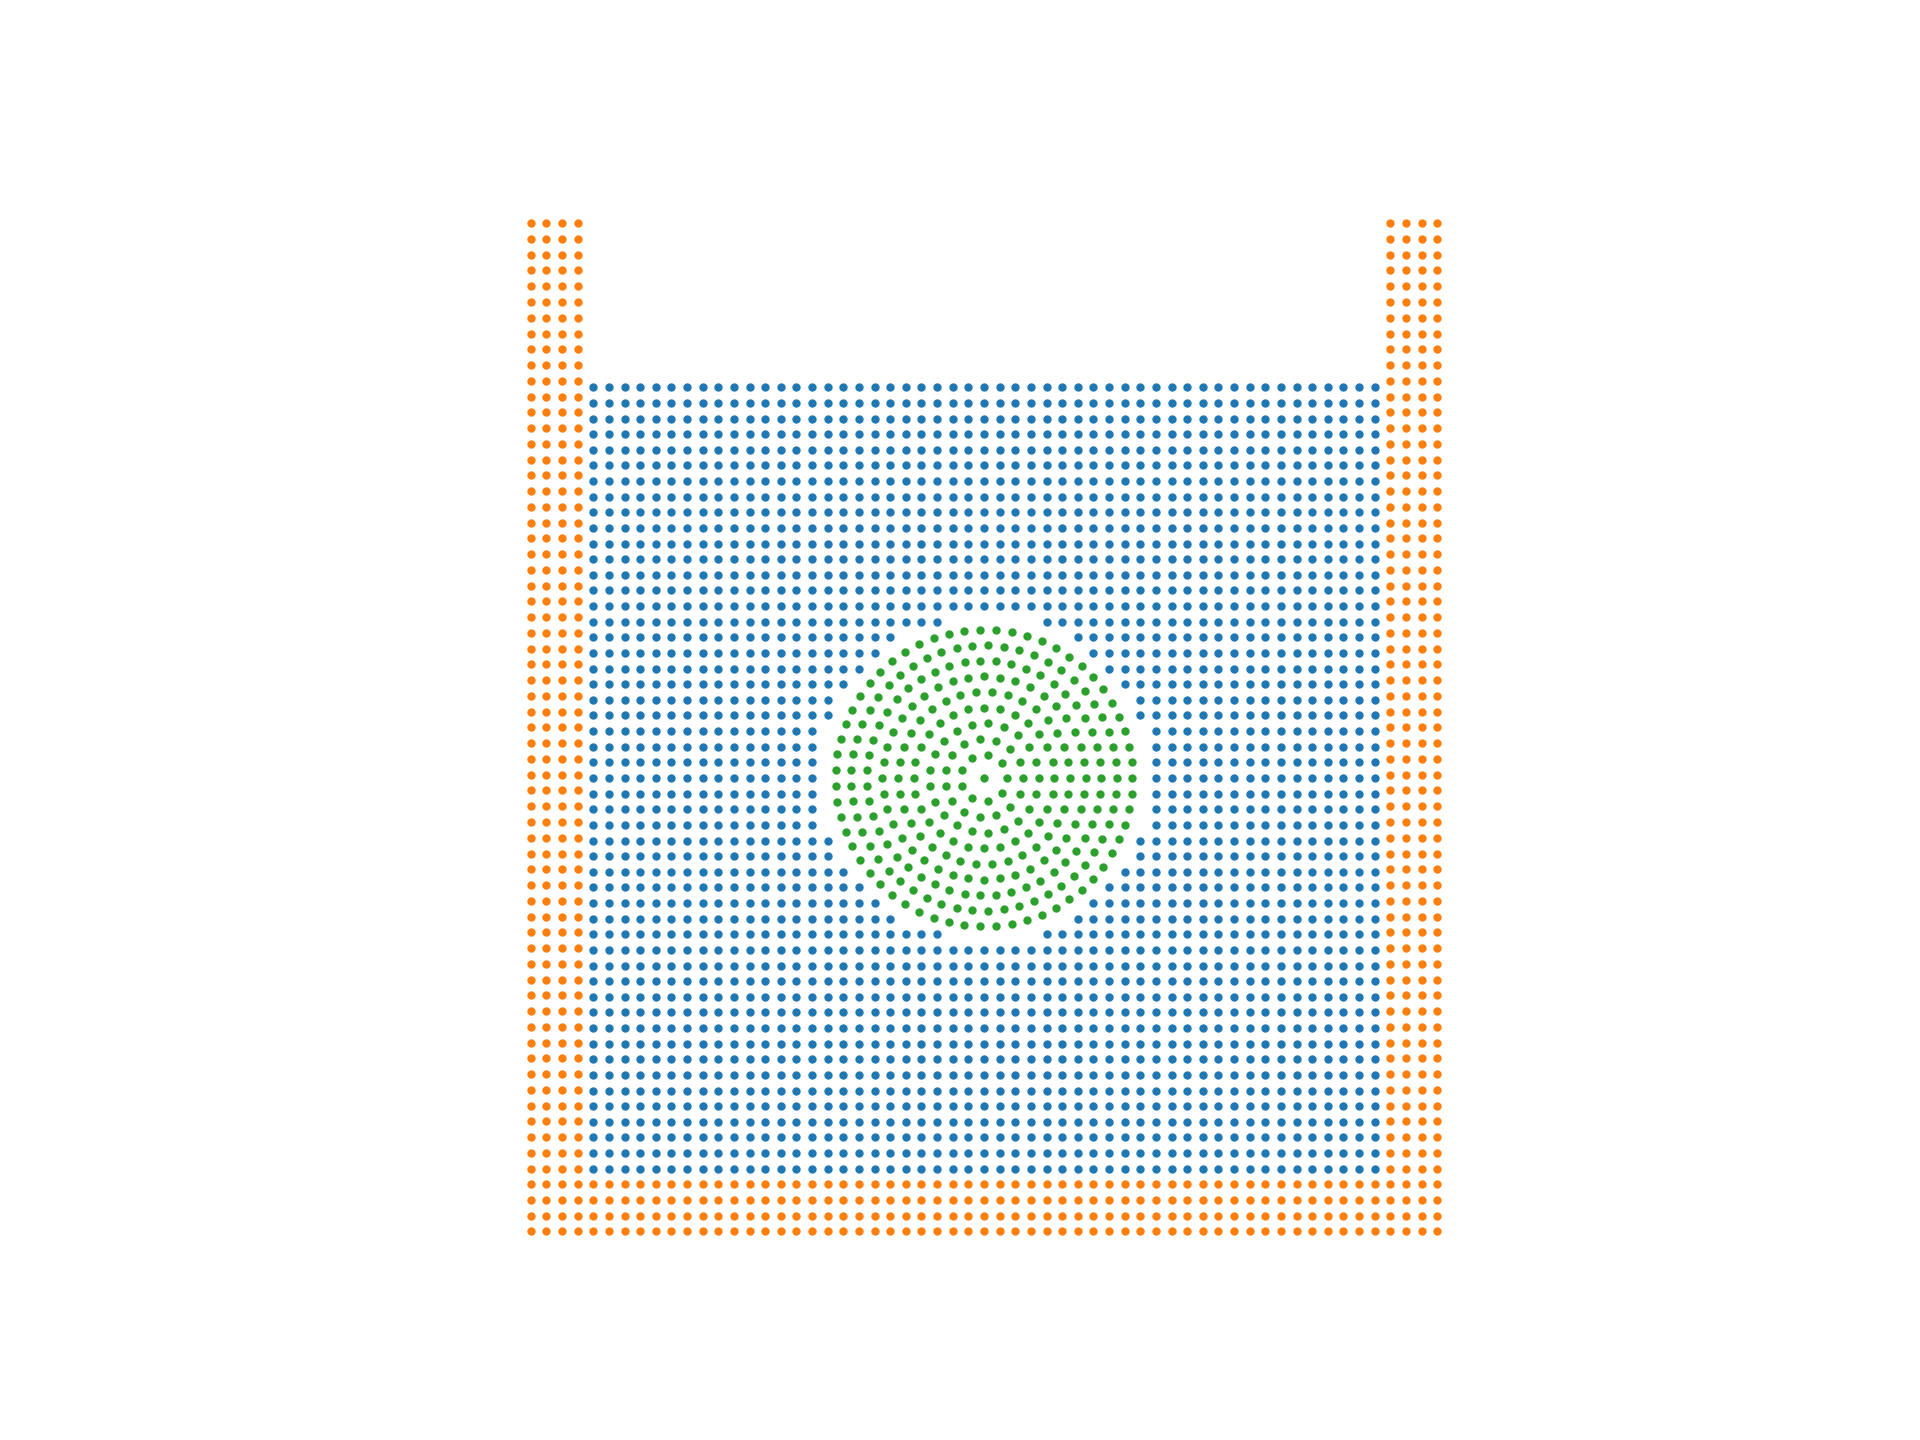
\includegraphics[width=1.0\textwidth]{images/hs_tank_with_spherical_particles_sph_0_6}
    \subcaption{t = $9.9$ s}\label{fig:1-mixing-1-c}
  \end{subfigure}
  \caption{}
\label{fig:xxxx}
\end{figure}


\FloatBarrier%
\section{Results}


\subsection*{Swelling model validation}

Put the particle at steady, and swell it. Mention the rise in the free surface
level, and discuss archimedes principle to validate.


\subsection*{Single particle Archimedes principle}

Put the particle at steady, and swell it. Mention the rise in the free surface
level, and discuss archimedes principle to validate.

\begin{figure}[!htpb]
  \centering
    \includegraphics[width=0.45\textwidth]{figures/dinesh_2024_single_particle_swelling_volume_change_benchmark/volume_change_vs_t}
  \caption{}
\label{fig:}
\end{figure}

\begin{figure}[!htpb]
  \centering
  \begin{subfigure}{0.48\textwidth}
    \centering
    \includegraphics[width=0.45\textwidth]{figures/dinesh_2024_single_particle_swelling_volume_change_benchmark/N_15/time0}
    \subcaption{t = $3$ s}\label{fig:1-mixing-1-a}
  \end{subfigure}
  \begin{subfigure}{0.48\textwidth}
    \centering
    \includegraphics[width=0.45\textwidth]{figures/dinesh_2024_single_particle_swelling_volume_change_benchmark/N_15/time1}
    \subcaption{t = $6$ s}\label{fig:1-mixing-1-b}
  \end{subfigure}

  \begin{subfigure}{0.48\textwidth}
    \centering
    \includegraphics[width=0.45\textwidth]{figures/dinesh_2024_single_particle_swelling_volume_change_benchmark/N_15/time2}
    \subcaption{t = $9.9$ s}\label{fig:1-mixing-1-c}
  \end{subfigure}
  \begin{subfigure}{0.48\textwidth}
    \centering
    \includegraphics[width=0.45\textwidth]{figures/dinesh_2024_single_particle_swelling_volume_change_benchmark/N_15/time3}
    \subcaption{t = $9.9$ s}\label{fig:1-mixing-1-c}
  \end{subfigure}
  \caption{}
\label{fig:xxxx}
\end{figure}


\subsection*{1000 particles James simulation}

\subsection*{Binary particles simulation}


\FloatBarrier%
\section{Conclusions}
\label{sec:conclusions}

Influence of the cohesion among the particles on the mixing behaviour among
the particles can be studied as a furture work. Mixing behaviour with
different densities and different radius in place can be studied.


% \section*{References}


\bibliographystyle{model6-num-names}
\bibliography{references}
\end{document}

% ============================
% Table template for reference
% ============================
% \begin{table}[!ht]
%   \centering
%   \begin{tabular}[!ht]{ll}
%     \toprule
%     Quantity & Values\\
%     \midrule
%     $L$, length of the domain & 1 m \\
%     Time of simulation & 2.5 s \\
%     $c_s$ & 10 m/s \\
%     $\rho_0$, reference density & 1 kg/m\textsuperscript{3} \\
%     Reynolds number & 200 \& 1000 \\
%     Resolution, $L/\Delta x_{\max} : L/\Delta x_{\min}$ & $[100:200]$ \& $[150:300]$\\
%     Smoothing length factor, $h/\Delta x$ & 1.0\\
%     \bottomrule
%   \end{tabular}
%   \caption{Parameters used for the Taylor-Green vortex problem.}%
%   \label{tab:tgv-params}
% \end{table}

%%% Local Variables:
%%% mode: latex
%%% TeX-master: "paper"
%%% fill-column: 78
%%% End:
